\documentclass[12pt]{article}

\usepackage[utf8]{inputenc}	%Encoding UTF8 per accenti
\usepackage{pdflscape} % per pagine landscape

\usepackage[T1]{fontenc}

\usepackage[italian]{babel}

\usepackage[onehalfspacing]{setspace}	%Interlinea di 1.5

\usepackage[hyperfootnotes=false]{hyperref}	%Pacchetto per coll. ipertestuali

\usepackage{tabularx}
\usepackage{longtable,array} %Per Tabelle potenzialmente multipagina
\usepackage{fancyhdr}  % per gli header e footer
\usepackage{graphicx}  %per le immagini
\usepackage{flafter}
\usepackage{listings} %per i listati di codice
\usepackage[font=small,labelfont=bf]{caption}

\usepackage{framed}

\usepackage[headheight=2cm, headsep=0.5cm, a4paper, margin=3cm]{geometry}
\usepackage[bottom]{footmisc}

\hypersetup{colorlinks=true}		%Configurazione colore link documento
\hypersetup{linkcolor= blue}
\renewcommand\UrlFont{\color{blue}\rmfamily\itshape} %Forzato colore blu su tutti i link ESTERNI

\usepackage[dvipsnames,table]{xcolor}
\definecolor{bluelogo}{HTML}{415A66}
\definecolor{grigio}{HTML}{D0D0D0}
\usepackage{makecell}

\renewcommand{\footrulewidth}{0.1pt}
\newcommand{\glossario}{\textsubscript{G} }

\usepackage{fancyhdr}
\usepackage{lastpage}
 
\pagestyle{fancy}

\fancyhf{}

\lhead{
\includegraphics[scale=0.08]{./images/logo.png}}
\rhead{\rightmark}

\lfoot{Piano di Progetto v2.0.0}
\cfoot{}
\rfoot{Pagina \thepage \hspace{1pt} di \pageref*{LastPage}}

\makeindex
\setcounter{secnumdepth}{4}
\setcounter{tocdepth}{4}

%\lhead{
\includegraphics[scale=0.08]{./images/logo.png}}
%\usepackage[headheight=2cm, headsep=0.5cm, a4paper, margin=3cm]{geometry}

\newcolumntype{C}[1]{>{\centering\arraybackslash}m{#1}}
\usepackage{eurosym}

\usepackage{grffile}
\usepackage{float}



\begin{document}
\begin{titlepage}
\thispagestyle{empty}
\pagenumbering{gobble}

\begin{center}


\includegraphics[scale=0.3]{./images/logo.png} 

\large \textbf{Agents of S.W.E. - Progetto "G\&B"}
\vfill
\Huge \textbf{Analisi dei Requisiti}
\vfill
\large
\renewcommand{\arraystretch}{1.3}
\begin{tabular}{r|l}
\textbf{Versione} & 2.0.7\\
\textbf{Approvazione} & Diego Mazzalovo\\
\textbf{Redazione} & \parbox[t]{5cm}{Luca Violato\\Marco Chilese\\Bogdan Stanciu\\Matteo Slanzi\\ Carlotta Segna}\\
\textbf{Verifica} & \parbox[t]{5cm}{Marco Favaro}\\
\textbf{Stato} & Approvato\\
\textbf{Uso} & Esterno\\
\textbf{Destinato a} & \parbox[t]{5cm}{Agents of S.W.E. \\Prof. Tullio Vardanega\\Prof. Riccardo Cardin \\ Zucchetti S.p.A.}
\end{tabular}
\vfill
\small
\texttt{agentsofswe@gmail.com}
\end{center}
\end{titlepage}

\pagebreak

\pagenumbering{arabic}

\section{Changelog}

\begin{center}
\begin{longtable}[c]{|m{.11\textwidth}|m{.13\textwidth}|m{.1\textwidth}|m{.19\textwidth}|p{.33\textwidth}|}
\hline
\rowcolor{bluelogo}\textbf{\textcolor{white}{Versione}} & \textbf{\textcolor{white}{Data}} & \textbf{\textcolor{white}{Autore}} & \textbf{\textcolor{white}{Ruolo}} & \textbf{\textcolor{white}{Descrizione}}\\
\hline \hline
\endfirsthead
0.0.1 & 2018-11-23 & Luca Violato & Amministratore & Strutturazione del Documento \\
\hline
\rowcolor{grigio} 0.0.2 & 2018-12-18 & Carlotta Segna & Responsabile & Standardizzazione tabella \\
\hline
\caption{Changelog del documento}
\end{longtable}
\end{center}
\newpage


\tableofcontents

% Inclusione degli indici di tabelle e immagini
\listoftables
\listoffigures

\pagebreak

%\pagenumbering{arabic}

\pagebreak

\section{Introduzione}\label{Intro}

\subsection{Scopo del Documento}
Il presente documento è stato realizzato con lo scopo di presentare le funzionalità del prodotto e spiegare, in modo intuitivo ma preciso, le modalità di utilizzo del plug-in \textit{G\&B}.

\subsection{Scopo del Prodotto}\label{ScopoProdotto}
Lo scopo del prodotto è la creazione di un plug-in per la piattaforma open source di visualizzazione e gestione dati, denominata \textit{Grafana}\glossario, con l'obiettivo di creare un sistema di alert\glossario dinamico per monitorare la "liveliness\glossario" del sistema a supporto dei processi DevOps\glossario e per consigliare interventi nel sistema di produzione del software. In particolare, il plug-in utilizzerà dati in input forniti ad intervalli regolari o con continuità, ad una rete bayesiana\glossario per stimare la probabilità di alcuni eventi, segnalandone quindi il rischio in modo dinamico, prevenendo situazioni di stallo.



\pagebreak

\section{Descrizione del Prodotto}\label{DescrizioneProdotto}

\subsection{Caratteristiche del Prodotto}\label{CaratteristicheProdotto}
Lo scopo del progetto è quello di realizzare un plug-in\glossario per \textit{Grafana}\glossario, in grado di utilizzare una rete bayesiana\glossario, definita ad hoc in formato \textit{JSON}\glossario, per stimare la probabilità che alcuni eventi si possano verificare o meno.\\
In particolare, deve essere possibile registrare i dati di un particolare ambiente, ad esempio tutti i dati di PC quali percentuale d'uso della CPU, pressione di memoria, utilizzo del disco ecc., che verranno poi visualizzati in pannelli di una dashboard\glossario. Tra tali pannelli dovrà esserne presente uno in cui visualizzare la probabilità di determinati eventi.\\
La probabilità di eventi definiti in sede di progettazione, viene stimata dalla rete bayesiana che, utilizzando i dati di ambiente, potrà avanzare delle ipotesi sugli eventi in atto. Un esempio: in un contesto di un calcolatore a cui è affidata la gestione di un complesso database\glossario, se si rilevasse un elevato uso della CPU, un'alta percentuale di memoria RAM occupata, ma un basso tasso di scrittura su disco, mediante parametri prefissati, la rete potrà ipotizzare con una probabilità $x$ che si stanno eseguendo delle "query\glossario lente"\footnote{Si intende query malformate che richiedono un eccessivo dispendio di risorse.}, permettendo quindi l'intervento da parte dei gestori del database in modo da non sprecare risorse preziose.\\
La stima delle probabilità deve essere eseguita secondo regole temporali prefissate. Ciò significa che il plug-in continuerà a registrare dati provenienti dall'ambiente e che ad ogni intervallo di tempo $t$ eseguirà un ricalcolo delle probabilità, fornendo di conseguenza appropriati alert, ove necessario.\\
La rete bayesiana in formato \textit{JSON}, menzionata sopra, può essere sviluppata tramite la libreria \textit{jsbayes}\glossario, indicata dalla proponente.\\
Inoltre, deve essere possibile caricare diverse tipologie di reti (che si differenziano per topologia, dati osservati e fenomeni monitorati) all'interno del plug-in, a seconda degli eventi che si intende intercettare. Deve essere poi possibile fornire alla rete nuovi dati provenienti da nodi non collegati al flusso di dati che si stanno captando ad intervalli regolari.

\subsection{Obiettivi del Prodotto}\label{ObiettiviProdotto}
L'obiettivo del progetto è la realizzazione di un plug-in, avente le caratteristiche descritte in §\ref{CaratteristicheProdotto}, che consenta agli utenti interessati di monitorare un flusso dati con maggiore efficienza ed efficacia rispetto al normale utilizzo della piattaforma \textit{Grafana}. Più nel dettaglio lo scopo finale del prodotto è quello di fornire all'utente dati aggiuntivi, ed eventualmente alert ad essi collegati, attraverso l'uso di un'apposita rete bayesiana.\\
Un esempio più concreto del beneficio derivato da un corretto utilizzo del prodotto è stato discusso in riunione esterna con l'azienda proponente: monitorando un determinato flusso dati con il plug-in "G\&B" è possibile ottenere assunzioni probabilistiche sulle cause che stanno a monte di determinate problematiche, le quali possono essere riscontrate attraverso il normale utilizzo di \textit{Grafana}, come ad esempio un'elevata pressione di memoria oppure un utilizzo della CPU anormale.

\subsection{Caratteristiche degli Utenti}\label{CaratteristicheUtenti}
Il plug-in di \textit{Grafana} "G\&B" è caratterizzato da un ambito di utilizzo, ed un relativo bacino di utenza, singolarmente ristretto. Il prodotto finale è rivolto ai soli utenti già registrati presso la piattaforma \textit{Grafana} che desiderano monitorare un determinato flusso dati attraverso l'uso di una qualche rete bayesiana in loro possesso.

\subsection{Vincoli Progettuali}\label{VincoliProgettuali}
L'implementazione finale del prodotto "G\&B" deve realizzare un plug-in per la piattaforma \textit{Grafana} con le caratteristiche descritte in §\ref{CaratteristicheProdotto} e che soddisfi gli obiettivi presentati in §\ref{ObiettiviProdotto} rispettando i seguenti vincoli:
\begin{itemize}
\item \textbf{Requisiti Minimi Obbligatori:}
	\begin{enumerate}
	\item Leggere la definizione della rete bayesiana da un file in formato \textit{.JSON};
	\item Associare alcuni nodi della rete ad un flusso di dati presente in \textit{Grafana};
	\item Applicare il ricalcolo delle probabilità della rete secondo regole temporali prestabilite;
	\item Fornire nuovi dati al sistema di \textit{Grafana} derivati dai nodi della rete non collegati al flusso di monitoraggio;
	\item Rendere disponibili i dati al sistema di creazione di grafici e dashboard per la loro visualizzazione.
	\end{enumerate}
\item \textbf{Requisiti Opzionali:}
	\begin{enumerate}
	\item Possibilità di definire alert in base a livelli di soglia raggiunti dai nodi non collegati al flusso dati;
	\item Possibilità di disegnare la rete bayesiana con un editor grafico;
	\item Possibilità di applicare più reti bayesiane ad oggetti di monitoraggio diversi;
	\item Possibilità di creare la rete bayesiana a partire da dati raccolti sul campo;
	\item Identificare altri metodi di IA applicabili.
	\end{enumerate}
\item \textbf{Tecnologie Richieste:}
	\begin{itemize}
	\item \textit{ECMAScript} 6 per lo sviluppo di plug-in per \textit{Grafana};
	\item \textit{JSON} per la definizione della rete bayesiana;
	\item \textit{Jsbayes} (libreria open-source) per la gestione dei calcoli della rete bayesiana.
	\end{itemize}
\end{itemize}
 


\pagebreak
\rhead{3 Casi d'Uso}

\section{Casi d'Uso}\label{CasiUso}
\subsection{Introduzione}\label{CasiUso_Introduzione}
Nella seguente sezione verranno identificati i casi d'uso che abbiamo individuato.\\
Il numero di casi che abbiamo analizzato è limitato poiché il plug-in fornisce funzionalità aggiuntive ad una piattaforma preesistente, per la quale non è fornita documentazione in quanto già disponibile presso il sito web del fornitore della piattaforma: \textit{Grafana Labs}.

\subsection{Attori}\label{Attori}
È importante notare che il numero esiguo di differenti attori che possono approcciarsi al prodotto in esame è principalmente dovuto al fatto che, essendo il progetto "G\&B" un plug-in di un sistema indipendente, poche tipologie di utenti possono effettivamente approcciarsi al prodotto finale.\\
È altrettanto importante sottolineare che il sistema di registrazione ed autenticazione dell'utente viene gestito interamente dal sistema \textit{Grafana}, dal momento che, ovviamente, il prodotto finale non avrà una funzionalità di autenticazione interna.

\subsubsection*{Attori Primari}
\begin{itemize}
\item \textbf{Utente:} si riferisce ad un generico utente che ha effettuato l'autenticazione al sistema \textit{Grafana}. È l'unica tipologia di utente con facoltà di interagire con il prodotto, in quanto questo risulta essere un plug-in.
\end{itemize}

\subsubsection*{Attori Secondari}
\begin{itemize}
\item \textbf{Piattaforma \textit{Grafana}:} sistema di monitoraggio di flusso dati, di cui il prodotto da realizzare è un plug-in. Consente agli utenti autenticati, attraverso funzionalità proprie, di realizzare grafici ed alert riferiti a dati forniti dal plug-in.
\end{itemize}

\begin{comment}
\begin{itemize}
	\item \textbf{Attore Primario:}
	\item \textbf{Precondizioni:}
	\begin{enumerate}
 		\item
	\end{enumerate}
	\item \textbf{Postcondizioni:}
	\begin{enumerate}
		\item
	\end{enumerate}
	\item \textbf{Scenario Principale:}
	\begin{enumerate}
		\item
	\end{enumerate}
	\item \textbf{Estensioni:}
\end{itemize}
\end{comment}

\subsection{Panoramica Casi d'Uso}\label{PanoramicaUC}
\begin{figure}[H]
	\begin{center}
		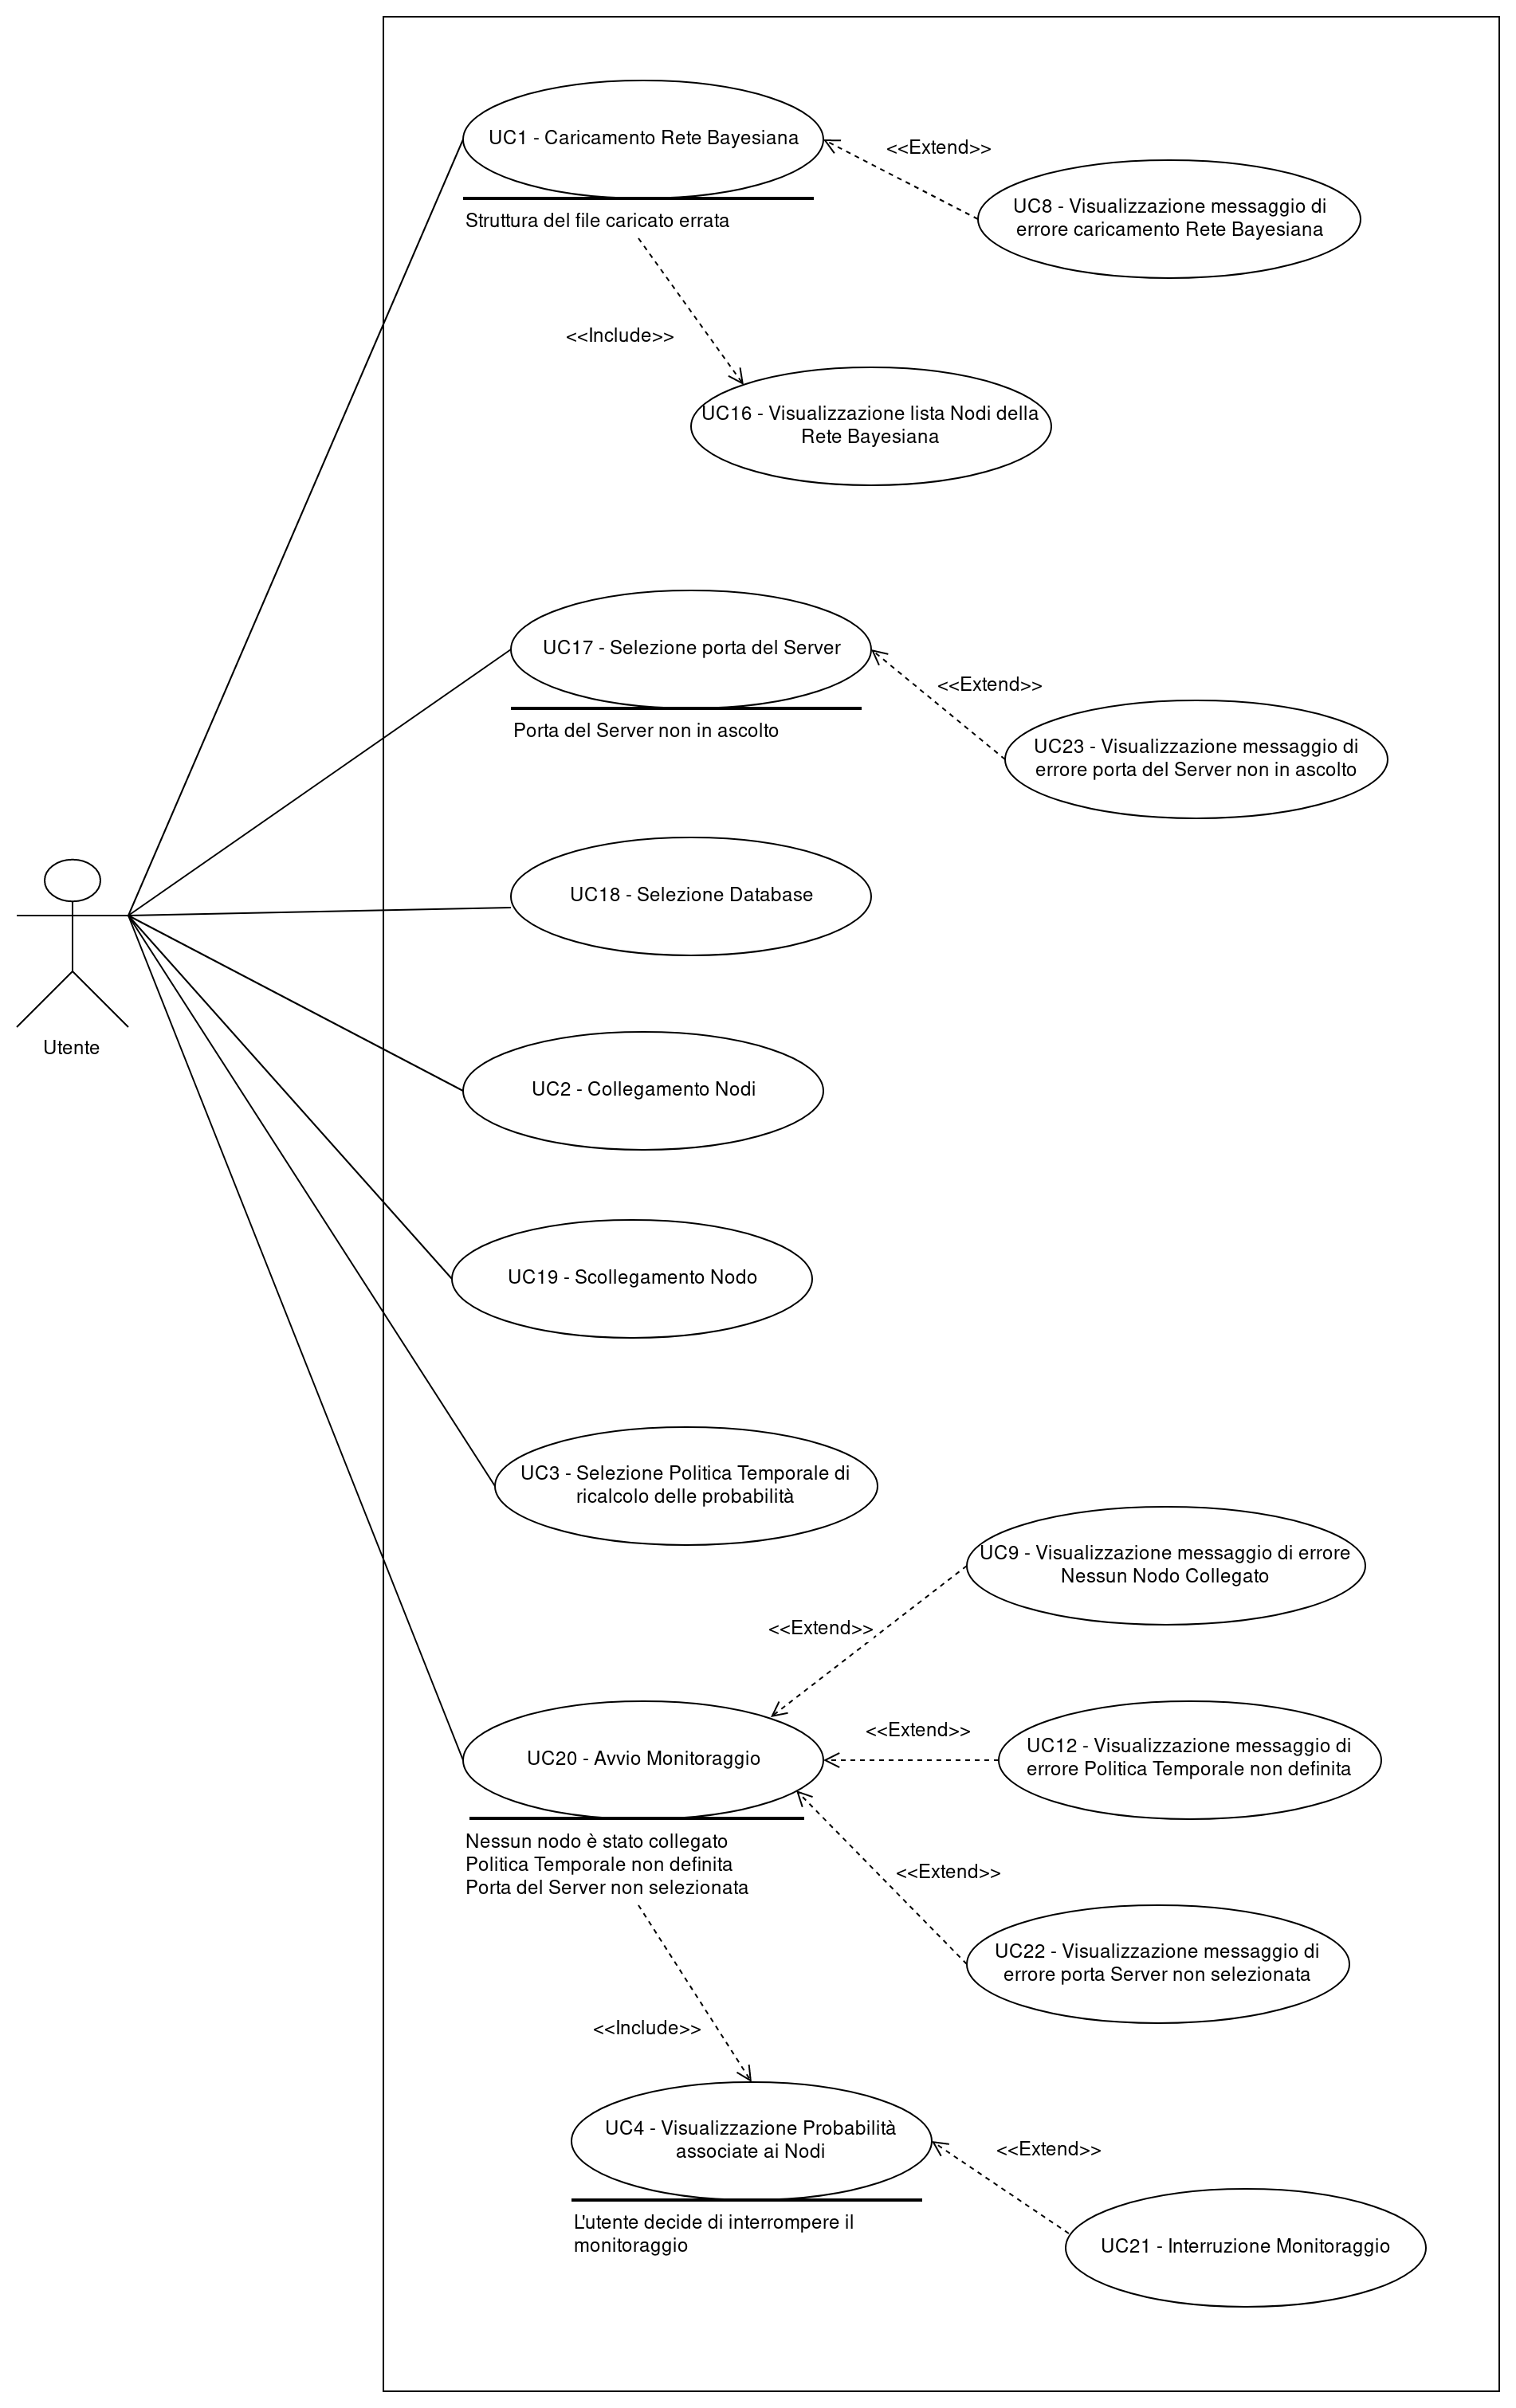
\includegraphics[scale=0.18]{./images/VistaUC.png}
		 \caption{Panoramica dei Casi d'Uso basilari}
	\end{center}
\end{figure}

\pagebreak
\subsection{UC1 - Caricamento Rete Bayesiana}\label{UC1}
\begin{figure}[H]
	\begin{center}
		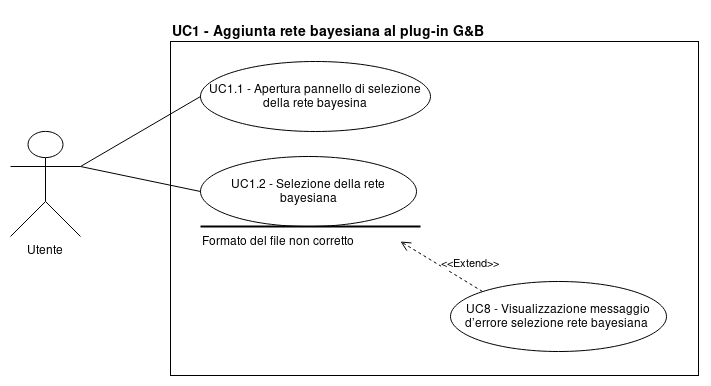
\includegraphics[scale=0.5]{./images/UC1.png}
		 \caption{UC1 - Aggiunta della Rete Bayesiana al Plug-in G\&B}
	\end{center}
\end{figure}

\begin{itemize}
	\item \textbf{Attore Primario}: Utente;
	\item \textbf{Precondizioni}:
		\begin{enumerate}
			\item L'utente deve aver effettuato il login nella piattaforma \textit{Grafana}, deve aver selezionato una dashboard e aggiunto il pannello "G\&B";
			\item L'utente deve aver correttamente configurato la connessione al server (\hyperref[UC17]{UC17 (§\ref*{UC17})}).
		\end{enumerate}
	\item \textbf{Postcondizioni}:
	\begin{enumerate}
		\item L'utente ha aggiunto la rete bayesiana al plug-in;
		\item L'utente visualizza il pulsante denominato "Avvio Monitoraggio".
	\end{enumerate}
	\item \textbf{Scenario Principale:}
	\begin{enumerate}
		\item (\hyperref[UC1.1]{UC1.1 (§\ref*{UC1.1})}) L'utente apre il pannello di selezione della rete bayesiana da caricare attraverso il click del pulsante "Seleziona Rete";
		\item (\hyperref[UC1.2]{UC1.2 (§\ref*{UC1.2})}) L'utente seleziona la rete bayesiana che desidera caricare.
	\end{enumerate}
	\item \textbf{Estensioni:} \hyperref[UC8]{UC8 (§\ref*{UC8})} estende \hyperref[UC1.2]{UC1.2 (§\ref*{UC1.2})}: l'utente visualizza un messaggio di errore nel caso in cui l'operazione non sia andata a buon fine.
	\item \textbf{Inclusioni:} UC1 include \hyperref[UC16]{UC16 (§\ref*{UC16})}: Viene visualizzata la lista di nodi di cui la rete bayesiana caricata è costituita.
\end{itemize}

\pagebreak

\subsubsection{UC1.1 - Apertura Pannello di Selezione del file}\label{UC1.1}
\begin{itemize}
	\item \textbf{Attore Primario}: Utente;
	\item \textbf{Precondizioni}: l'utente visualizza il pannello "G\&B" nella dashboard.
	\item \textbf{Postcondizioni}: l'utente ha cliccato il bottone con etichetta "Seleziona Rete" e visualizza il pannello per la selezione del file della rete;
	\item \textbf{Scenario Principale}: l'utente clicca il pulsante con etichetta "Seleziona Rete".
\end{itemize}


\subsubsection{UC1.2 - Selezione della Rete Bayesiana}\label{UC1.2}
\begin{itemize}
	\item \textbf{Attore Primario}: Utente;
	\item \textbf{Precondizioni}: l'utente ha cliccato il bottone con etichetta "Seleziona Rete";
	\item \textbf{Postcondizioni}: l'utente ha caricato con successo il file \textit{JSON} contente la definizione della rete bayesiana;
	\item \textbf{Scenario Principale}:
	\begin{enumerate}
		\item L'utente seleziona dalla finestra il file da importare;
		\item L'utente clicca il pulsante con etichetta "Apri".
	\end{enumerate}
	\item \textbf{Estensioni:} \hyperref[UC8]{UC8 (§\ref*{UC8})}: l'utente visualizza un messaggio di errore nel caso in cui l'operazione di caricamento del file non sia andata a buon fine.
\end{itemize}

\pagebreak

\subsection{UC2 - Collegamento Nodi al Flusso Dati}\label{UC2}
\begin{figure}[H]
\centering
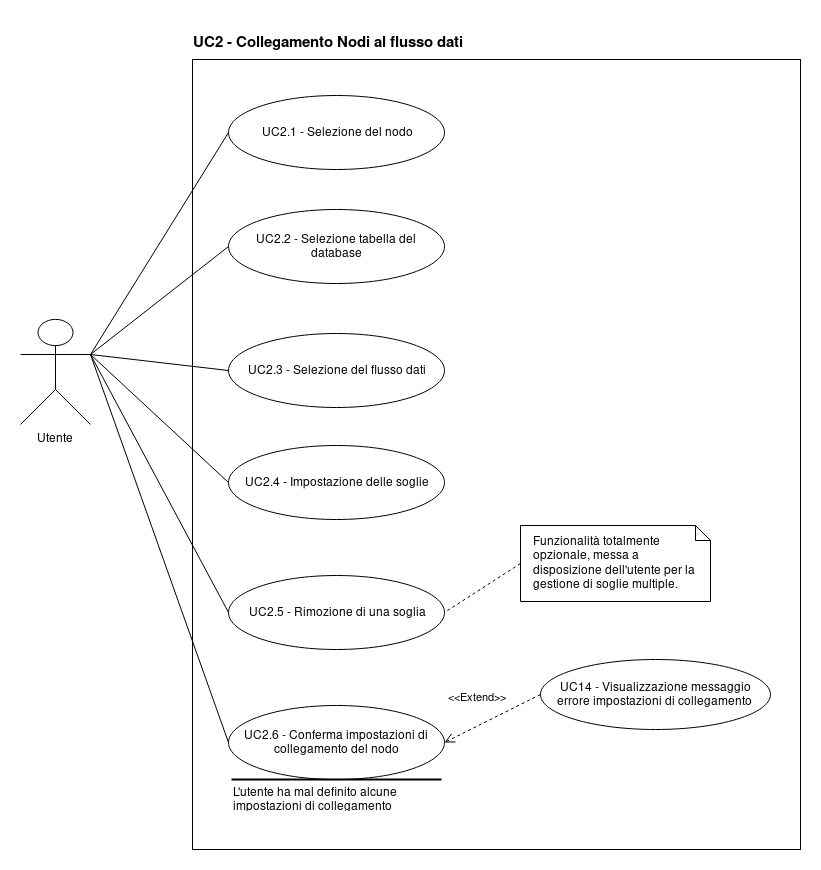
\includegraphics[scale=0.5]{./images/UC2.png}
\caption{UC2 - Collegamento Nodi al Flusso Dati}
\end{figure}

\begin{itemize}
\item \textbf{Attore Primario}: Utente;
\item \textbf{Precondizioni}:
\begin{enumerate}
	\item L'utente ha caricato con successo la rete bayesiana (\hyperref[UC1]{UC1(§\ref*{UC1})});
	\item L'utente visualizza la lista di nodi di cui la rete bayesiana è costituita	(\hyperref[UC16]{UC16 (§\ref*{UC16})}).
\end{enumerate}
\item \textbf{Postcondizione}: L'utente ha collegato correttamente uno o più nodi ad un flusso dati, definendone le soglie per i rispettivi stati.
\item \textbf{Scenario Principale}:
 \begin{enumerate}
 \item (\hyperref[UC2.1]{UC2.1 (§\ref*{UC2.1})}) Selezione del Nodo;
 \item (\hyperref[UC2.2]{UC2.2 (§\ref*{UC2.2})}) Selezione della tabella del database;
 \item (\hyperref[UC2.3]{UC2.3 (§\ref*{UC2.3})}) Selezione del flusso dati;
 \item (\hyperref[UC2.4]{UC2.4 (§\ref*{UC2.4})}) Impostazione delle soglie;
 \item (\hyperref[UC2.5]{UC2.5 (§\ref*{UC2.5})}) Rimozione di una soglia;
 \item (\hyperref[UC2.6]{UC2.6 (§\ref*{UC2.6})}) Conferma impostazioni di collegamento del nodo;
 \end{enumerate}
\item \textbf{Estensioni:} \hyperref[UC14]{UC14 (§\ref*{UC14})} estende \hyperref[UC2.6]{UC2.6 (§\ref*{UC2.6})}: l'utente visualizza un messaggio di errore nel caso in cui non abbia definito correttamente le impostazioni di collegamento.
\end{itemize}

\subsubsection{UC2.1 - Selezione del Nodo}\label{UC2.1}
\begin{itemize}
\item \textbf{Attore Primario:} Utente;
\item \textbf{Precondizione:} l'utente visualizza la lista di nodi di cui la rete bayesiana è costituita ed il 	corrispondente stato (\hyperref[UC16]{UC16 (§\ref*{UC16})});
\item \textbf{Postcondizione:} l'utente visualizza una finestra contenente le impostazioni di collegamento del nodo selezionato;
\item \textbf{Scenario Principale:} l'utente clicca il nominativo del nodo che desidera collegare al flusso dati.
\end{itemize}

\subsubsection{UC2.2 - Selezione Tabella Database}\label{UC2.2}
\begin{itemize}
\item \textbf{Attore Primario:} Utente;
\item \textbf{Precondizione:} l'utente ha selezionato il nodo che desidera collegare al flusso dati 					(\hyperref[UC2.1]{UC2.1 (§\ref*{UC2.1})});
\item \textbf{Postcondizioni:}
	\begin{enumerate}
	\item L'utente ha selezionato la tabella del database contente i flussi dati da selezionare;
	\item In base alla tabella selezionata cambia contestualemnte il contenuto del menù a tendina per la selezione del flusso dati (\hyperref[UC2.3]{UC2.3 (§\ref*{UC2.3})});
	\end{enumerate}
\item \textbf{Scenario Principale:} l'utente seleziona, attraverso un menù a tendina, il flusso dati a cui desidera collegare il nodo in esame.
\end{itemize}

\subsubsection{UC2.3 - Selezione del Flusso Dati}\label{UC2.3}
\begin{itemize}
	\item \textbf{Attore Primario:} Utente;
	\item \textbf{Precondizione:} l'utente ha selezionato il nodo che desidera collegare al flusso dati 						(\hyperref[UC2.1]{UC2.1 (§\ref*{UC2.1})});
	\item \textbf{Postcondizioni:} l'utente ha selezionato il flusso dati a cui collegare il nodo desiderato;
	\item \textbf{Scenario Principale:} l'utente seleziona, attraverso un menù a tendina, il flusso dati a cui desidera collegare il nodo in esame.
\end{itemize}

\pagebreak

\subsubsection{UC2.4 - Impostazione soglie}\label{UC2.4}

\begin{figure}[H]
\centering
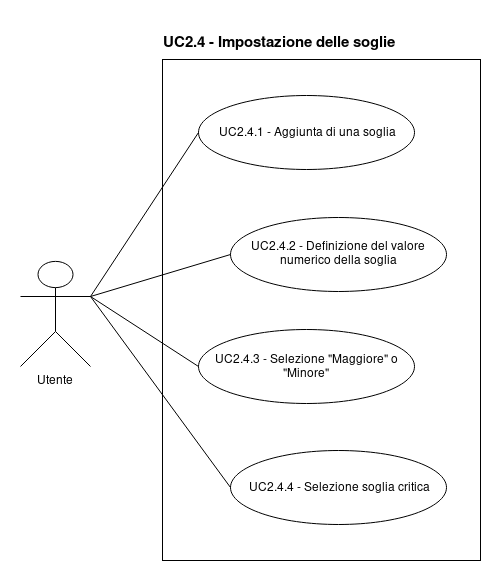
\includegraphics[scale=0.5]{./images/UC2-4.png}
\caption{UC2.4 - Impostazione delle soglie}
\end{figure}

\begin{itemize}
\item \textbf{Attore Primario:} Utente
\item \textbf{Precondizione:} l'utente ha selezionato il nodo che desidera collegare al flusso dati 					(\hyperref[UC2.1]{UC2.1 (§\ref*{UC2.1})});
\item \textbf{Postcondizione:} l'utente ha impostato, per ogni stato del nodo, una o più soglie, le quali hanno la funzionalità di definire gli insiemi di valori per i quali la probabilità associata allo stato in questione risulta pari al 100\%, mentre le probabilità associate agli altri stati risultano pari allo 0\%;
\item \textbf{Scenario Principale:}
	\begin{enumerate}
	\item (\hyperref[UC2.4.1]{UC2.4.1 (§\ref*{UC2.4.1})}) Aggiunta di una soglia;
	\item (\hyperref[UC2.4.2]{UC2.4.2 (§\ref*{UC2.4.2})}) Definizione del valore numerico della soglia;
	\item (\hyperref[UC2.4.3]{UC2.4.3 (§\ref*{UC2.4.3})}) Selezione "Maggiore" o "Minore";
	\item (\hyperref[UC2.4.4]{UC2.4.4 (§\ref*{UC2.4.4})}) Selezione soglia critica.
	\end{enumerate}
\end{itemize}

\paragraph{UC2.4.1 - Aggiunta di una soglia}\label{UC2.4.1}
\begin{itemize}
	\item \textbf{Attore Primario:} Utente;
	\item \textbf{Precondizioni:} l'utente ha selezionato il nodo che desidera collegare al flusso dati 					(\hyperref[UC2.1]{UC2.1 (§\ref*{UC2.1})});
	\item \textbf{Postcondizione:} l'utente visualizza i campi dati editabili da compilare per definire una soglia per lo stato in questione;
	\item \textbf{Scenario Principale:} l'utente aggiunge una soglia editabile per lo stato del nodo desiderato cliccando il pulsante "Aggiungi Soglia" posizionato accanto al nominativo dello stato. Se lo desidera l'utente può ripetere più volte l'operazione per lo stesso stato, aggiungendo così la possibilità di definire molteplici soglie per lo stesso stato.
\end{itemize}

\paragraph{UC2.4.2 - Definizione valore numerico della soglia}\label{UC2.4.2}
\begin{itemize}
	\item \textbf{Attore Primario:} Utente;
	\item \textbf{Precondizioni:} l'utente ha aggiunto una soglia (\hyperref[UC2.4.1]{UC2.4.1 (§\ref*{UC2.4.1})});
	\item \textbf{Postcondizioni:} l'utente ha definito il valore numerico della soglia;
	\item \textbf{Scenario Principale:} l'utente edita il campo dati cliccando sullo stesso e digitando il valore numerico che desidera associare alla soglia in esame.
\end{itemize}

\paragraph{UC2.4.3 - Selezione "Maggiore" o "Minore"}\label{UC2.4.3}
\begin{itemize}
	\item \textbf{Attore Primario:} Utente;
	\item \textbf{Precondizioni:} l'utente ha aggiunto una soglia (\hyperref[UC2.4.1]{UC2.4.1 (§\ref*{UC2.4.1})});
	\item \textbf{Postcondizioni:} l'utente ha selezionato il senso (">",">=","<" o "<=") attraverso cui interpretare l'insieme di valori di cui il valore di soglia (definito in \hyperref[UC2.4.2]{UC2.4.2 (§\ref*{UC2.4.2})}) rappresenta quindi rispettivamente il minimo o il massimo.
	\item \textbf{Scenario Principale:} l'utente seleziona, attraverso una casella a scelta multipla uno dei seguenti valori: ">",">=","<" o "<=".
\end{itemize}

\paragraph{UC2.4.4 - Selezione soglia critica}\label{UC2.4.4}
\begin{itemize}
	\item \textbf{Attore Primario:} Utente
	\item \textbf{Precondizioni:} l'utente ha aggiunto una soglia (\hyperref[UC2.4.1]{UC2.4.1 (§\ref*{UC2.4.1})});
	\item \textbf{Postcondizioni:} l'utente ha identificato la soglia come critica o meno.
	\item \textbf{Scenario Principale:} Per ogni stato del nodo l'utente seleziona, attraverso una checkbox, se la soglia definita sia critica o meno. Nel caso in cui si tratti di una soglia critica, qualora dovessero essere monitorati valori che la facciano scattare, si attiverebbe immediatamente l'attività di ricalcolo delle probabilità in sede di monitoraggio e visualizzazione dati (\hyperref[UC4]{UC4 (§\ref*{UC4})}).
\end{itemize}

\pagebreak

\subsubsection{UC2.5 - Rimozione di una soglia}\label{UC2.5}
\begin{itemize}
	\item \textbf{Attore Primario:} Utente
	\item \textbf{Precondizioni:} l'utente ha aggiunto una soglia (\hyperref[UC2.4.1]{UC2.4.1 (§\ref*{UC2.4.1})});
	\item \textbf{Postcondizioni:} l'utente ha rimosso la soglia.
	\item \textbf{Scenario Principale:} L'utente, se lo desidera, rimuove la soglia aggiunta in \hyperref[UC2.4.1]{UC2.4.1 (§\ref*{UC2.4.1})} cliccando il pulsante "Rimuovi".
\end{itemize}

\subsubsection{UC2.6 - Conferma impostazioni di collegamento del nodo}\label{UC2.6}
\begin{itemize}
\item \textbf{Attore Primario:} Utente;
\item \textbf{Precondizioni:} l'utente ha selezionato il nodo che desidera collegare al flusso dati 					(\hyperref[UC2.1]{UC2.1 (§\ref*{UC2.1})});
\item \textbf{Postcondizioni:}
	\begin{enumerate}
	\item La finestra, comparsa per consentire all'utente di compiere le operazioni necessarie al fine di collegare il 		nodo ad un flusso dati, scompare. L'utente visualizza nuovamente la lista dei nodi della rete bayesiana caricata;
	\item La checkbox corrispondente al nodo appena collegato passa allo stato "V", che rappresenta graficamente il fatto che il nodo è stato collegato al flusso dati;
	\item Accanto al nominativo del nodo appena collegato compare il pulsante "Scollega Nodo";
	\item L'utente, se lo desidera, può selezionare un altro nodo da collegare tornando quindi a \hyperref[UC2.1]{UC2.1 (§\ref*{UC2.1})}.
	\end{enumerate}
\item \textbf{Scenario Principale:} l'utente clicca il pulsante "Conferma";
\item \textbf{Estensioni:} \hyperref[UC14]{UC14 (§\ref*{UC14})}: nel caso in cui l'utente abbia commesso degli errori nella definizione delle impostazione di collegamento riceve un messaggio di errore.
\end{itemize}

\pagebreak

\subsection{UC3 - Selezione Politica Temporale di Ricalcolo delle Probabilità}\label{UC3}
\begin{figure}[H]
\centering
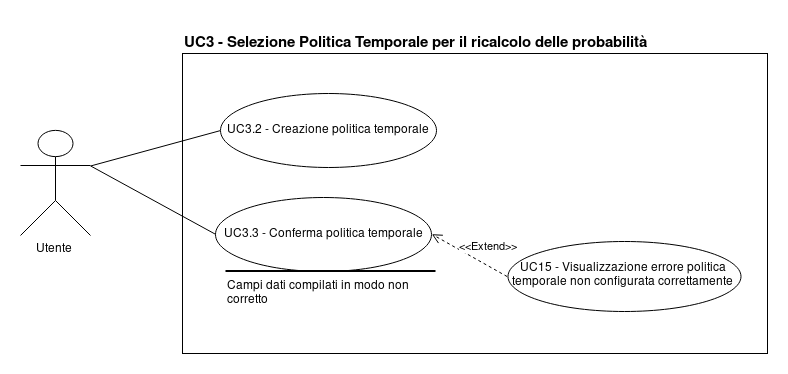
\includegraphics[scale=0.5]{./images/UC3.png}
\caption{UC3 - Selezione Politica Temporale di Ricalcolo delle Probabilità.}
\end{figure}

\begin{itemize}
	\item \textbf{Attore Primario}: Utente;
	\item \textbf{Precondizione}:
		\begin{enumerate}
			\item L'utente deve aver correttamente configurato la connessione al server (\hyperref[UC17]{UC17 (§\ref*{UC17})});
			\item L'utente si trova presso il pannello di configurazione della Politica Temporale, acceduto tramite il click del pulsante "Politica Temporale".
		\end{enumerate}
	\item \textbf{Postcondizione}: l'utente ha configurato con successo la politica temporale da lui creata, per il ricalcolo delle probabilità della rete bayesiana, caricata in (\hyperref[UC1]{UC1 (§\ref*{UC1})});
	\item \textbf{Scenario Principale:}
	\begin{enumerate}
		\item (\hyperref[UC3.1]{UC3.1 (§\ref*{UC3.1})}) L'utente crea una nuova politica temporale;
		\item (\hyperref[UC3.2]{UC3.2 (§\ref*{UC3.2})}) L'utente conferma la politica temporale realizzata.
	\end{enumerate}
	\item \textbf{Estensioni}: \hyperref[UC15]{UC15 (§\ref*{UC15})} estende \hyperref[UC3.2]{UC3.2 (§\ref*{UC3.2})}: l'utente visualizza un messaggio di errore nel caso in cui non abbia definito correttamente la politica temporale per il ricalcolo delle probabilità.
\end{itemize}

\pagebreak

\subsubsection{UC3.1 - Creazione Nuova Politica Temporale}\label{UC3.1}

\begin{itemize}
	\item \textbf{Attore Primario}: Utente;
	\item \textbf{Precondizione}: l'utente ha acceduto al pannello di creazione della politica temporale (\hyperref[UC3.1]{UC3.1 (§\ref*{UC3.1})});
	\item \textbf{Postcondizione}: l'utente ha realizzato la politica temporale per il ricalcolo delle probabilità desiderata;
	\item \textbf{Scenario Principale:}
	\begin{enumerate}
		\item L'utente visualizza due campi dati editabili che consentono la definizione di una politica temporale;
		\item L'utente inserisce, nel primo campo dati, il valore numerico del timeout ciclico per il ricalcolo delle probabilità condizionali associate ai nodi della rete bayesiana;
		\item L'utente seleziona l'unità di misura temporale, attraverso una casella a scelta multipla che rappresenta il secondo campo dati editabile.
	\end{enumerate}

\end{itemize}

\subsubsection{UC3.2 - Conferma Politica Temporale}\label{UC3.2}
\begin{itemize}
	\item \textbf{Attore Primario}: Utente;
	\item \textbf{Precondizione}: l'utente ha creato la politica temporale desiderata (\hyperref[UC3.2]{UC3.2 (§\ref*{UC3.2})});
	\item \textbf{Postcondizione}: l'utente ha confermato la politica temporale per il ricalcolo delle probabilità;
	\item \textbf{Scenario Principale}: l'utente clicca il pusante "Conferma".
	\item \textbf{Estensioni}: \hyperref[UC15]{UC15 (§\ref*{UC15})}: l'utente visualizza un messaggio di errore nel caso in cui non abbia collegato alcun nodo ad un flusso dati.
\end{itemize}

\newpage

\subsection{UC4 - Visualizzazione Probabilità Associate ai Nodi non Collegati al Flusso}\label{UC4}

\begin{itemize}
\item \textbf{Attore Primario}: Utente;
\item \textbf{Precondizione:} l'utente ha avviato correttamente il monitoraggio del flusso dati (\hyperref[UC20]{UC20 (§\ref*{UC20})}).
\item \textbf{Postcondizione:} il Sistema mantiene aggiornate, e visualizzabili da parte dell'utente, le misure di probabilità derivate dai nodi della rete bayesiana non collegati al flusso dati;
\item \textbf{Scenario Principale:} l'utente visualizza l'andamento delle probabilità dinamiche associate ai nodi 			della rete bayesiana non collegati direttamente al flusso dati. Il sistema aggiorna costantemente i dati forniti dalla rete bayesiana, effettuando l'operazione di ricalcolo delle probabilità associate ai nodi della rete non collegati al flusso dati. Tale operazione di ricalcolo delle probabilità viene eseguita allo scadere del timeout ciclico rappresentato dalla politica temporale stabilita in \hyperref[UC3]{UC3 (§\ref*{UC3})}, oppure, nel caso siano state definite in sede di collegamento nodi (\hyperref[UC2.3.4]{UC2.3.4 (§\ref*{UC2.3.4})}), ogni volta che una soglia critica viene attivata dai dati monitorati;
\item \textbf{Estensioni:} \textcolor{red}{UC21 (§\ref*{UC21})}: la visualizzazione dei dati viene interrotta nel 			caso in cui l'utente decida di modificare il collegamento dei nodi della rete bayesiana al flusso dati.
\end{itemize}

\pagebreak

\subsection{UC8 - Visualizzazione Messaggio d'Errore Selezione Rete Bayesiana}\label{UC8}
\begin{itemize}
\item \textbf{Attore Primario}: Utente;
\item \textbf{Precondizione}: l'utente ha selezionato una rete da aggiungere ed ha cliccato il pulsante "Aggiungi", per confermare la rete. La rete selezionata dall'utente è errata per formato o per struttura;
\item \textbf{Postcondizione}: l'utente visualizza l'errore, viene quindi riportato alla finestra di selezione del file della rete bayesiana (\hyperref[UC1.2]{UC1.2 (§\ref*{UC1.2})});
\item \textbf{Scenario Principale:}
	\begin{enumerate}
	\item L'utente visualizza un messaggio di errore in cui è segnalato il fatto che la struttura del file di definizione della rete bayesiana, caricato in (\hyperref[UC1.2]{UC1.2 (§\ref*{UC1.2})}, non è corretta;
	\item L'utente clicca il pulsante con etichetta "OK".
	\end{enumerate}
\end{itemize}

\pagebreak

\subsection{UC9 - Visualizzazione Messaggio di Errore Nessun Nodo Collegato}\label{UC9}
\begin{itemize}
\item \textbf{Attore Primario}: Utente;
\item \textbf{Precondizione}: l'utente ha avviato il monitoraggio (\hyperref[UC20]{UC20 (§\ref*{UC20})}), senza averne effettivamente collegato alcuno;
\item \textbf{Postcondizioni}:
	\begin{enumerate}
	\item l'utente visualizza l'errore;
	\item il monitoraggio dei dati non viene avviato;
	\end{enumerate}
\item \textbf{Scenario Principale}:
	\begin{enumerate}
	\item L'utente visualizza un messaggio di errore in cui è segnalato il fatto che non sia stato collegato alcun 				nodo al flusso dati (\hyperref[UC2]{UC2 (§\ref*{UC2})});
	\item L'utente clicca il pulsante con etichetta "OK".
	\end{enumerate}
\end{itemize}

\pagebreak

\subsection{UC12 - Visualizzazione Messaggio di Errore Politiche Temporali non Definite}\label{UC12}
\begin{itemize}
\item \textbf{Attore Primario}: Utente;
\item \textbf{Precondizione}: l'utente ha avviato il monitoraggio del flusso dati (\hyperref[UC20]{UC20 							(§\ref*{UC20})}), senza aver preventivamente definito correttamente alcuna politica temporale per il ricalcolo delle probabilità (\hyperref[UC3]{UC3 (§\ref*{UC3})}).
\item \textbf{Postcondizione}: l'utente visualizza l'errore;
\item \textbf{Scenario Principale}:
	\begin{enumerate}
	\item L'utente visualizza un messaggio di errore in cui è segnalato il fatto che non sia stata definita alcuna 				politica temporale per il ricalcolo delle probabilità;
	\item L'utente clicca il pulsante con etichetta "OK".
	\end{enumerate}
\end{itemize}

\newpage

\subsection{UC14 - Visualizzazione messaggio di errore Impostaziondi di Collegamento}\label{UC14}
\begin{itemize}
\item \textbf{Attore Primario}: Utente;
\item \textbf{Precondizione}: l'utente ha confermato le scelte per il collegamento di un dato nodo ad un flusso dati (\hyperref[UC2.6]{UC2.6 (§\ref*{UC2.6})}), avendo commesso alcuni errori durante la definizione delle impostazioni di collegamento;
\item \textbf{Postcondizioni}:
	\begin{enumerate}
	\item L'utente visualizza l'errore;
	\item Le scelte dell'utente non vengono confermate.
	\end{enumerate}
\item \textbf{Scenario Principale}:
	\begin{enumerate}
	\item L'utente visualizza un messaggio di errore in cui sono indicati gli errori commessi;
	\item L'utente clicca il pulsante con etichetta "OK".
	\end{enumerate}
\end{itemize}

\pagebreak

\subsection{UC15 - Visualizzazione Messaggio di Errore Politica Temporale non Configurata Correttamente}\label{UC15}
\begin{itemize}
	\item \textbf{Attore Primario}: Utente;
	\item \textbf{Precondizione}: l'utente ha confermato le scelte per la selezione di una politica temporale per il ricalcolo delle probabilità (\hyperref[UC3.2]{UC3.2 (§\ref*{UC3.2})}), senza averla definita correttamente (\hyperref[UC3.1]{UC3.1 (§\ref*{UC3.1})});
	\item \textbf{Postcondizioni}:
	\begin{enumerate}
		\item L'utente visualizza l'errore;
		\item La politica temporale non viene impostata.
	\end{enumerate}
	\item \textbf{Scenario Principale}:
	\begin{enumerate}
		\item L'utente visualizza un messaggio di errore in cui sono indicati gli errori commessi;
		\item L'utente clicca il pulsante con etichetta "OK".
	\end{enumerate}
\end{itemize}

\pagebreak

\subsection{UC16 - Visualizzazione della Lista dei Nodi della Rete Bayesiana}\label{UC16}
\begin{itemize}
	\item \textbf{Attore Primario:}  Utente
	\item \textbf{Precondizione:} l'utente ha caricato con successo la rete bayesiana (\hyperref[UC1]{UC1 	(§\ref*{UC1})});
	\item \textbf{Postcondizione:} l'utente visualizza la lista di nodi di cui la rete bayesiana è costituita;
	\item \textbf{Scenario Principale:}
	\begin{enumerate}
		\item L'utente visualizza la lista di nodi di cui la rete bayesiana, caricata in \hyperref[UC1]{UC1 									(§\ref*{UC1})}, è costituita. Ogni elemento della lista è formato da due componenti:
		\begin{itemize}
			\item Il nominativo del nodo stesso;
			\item Una checkbox\glossario la quale rappresenta lo stato di collegamento del nodo a cui è associata: verrà cisualizzata una "V" nel caso il nodo sia collegato ad un flusso dati, checkbox vuota altrimenti.
		\end{itemize}
	\end{enumerate}
\end{itemize}

\pagebreak

\subsection{UC17 - Configurazione Indirizzo e Porta del Server}\label{UC17}
\begin{figure}[H]
	\centering
	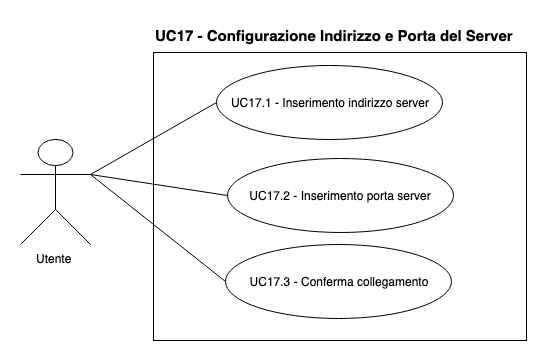
\includegraphics[scale=0.65]{./images/UC17.png}
	\caption{UC17 - Configurazione Indirizzo e Porta del Server.}
\end{figure}
\begin{itemize}
	\item \textbf{Attore Primario:}  Utente
	\item \textbf{Precondizione:}
		\begin{enumerate}
			\item L'utente ha aggiunto il pannello "G\&B" alla propria dashboard;
			\item L'utente si trova nella scheda "Server Setting" del menù "Edit" del pannello.
		\end{enumerate}
	\item \textbf{Postcondizione:} L'utente ha configurato i parametri di connessione al server;
	\item \textbf{Scenario Principale:}
	\begin{enumerate}
		\item (\hyperref[UC17.1]{UC17.1 (§\ref*{UC17.1})}) Inserimento indirizzo IP;
		\item (\hyperref[UC17.2]{UC17.2 (§\ref*{UC17.2})}) Inserimento porta;
		\item (\hyperref[UC17.3]{UC17.3 (§\ref*{UC17.3})}) Click conferma collegamento.
	\end{enumerate}
	\item \textbf{Estensioni}: si è verificato un errore di connessione: l'utente visualizza un messaggio che lo informa dell'avvenuto errore, invitandolo quindi a verificare la correttezza di indirizzo e/o porta, e clicca "OK" (\hyperref[UC22]{UC22 (§\ref*{UC22})});
	\item  \textbf{Inclusione}: (\hyperref[UC26]{UC26 (§\ref*{UC26})}) Visualizzazione notifica di avvenuto collegamento;
\end{itemize}

\subsubsection{UC17.1 - Inserimento Indirizzo Server}\label{UC17.1}
\begin{itemize}
	\item \textbf{Attore Primario:}  Utente
	\item \textbf{Precondizione:} L'utente si trova nella scheda "Server Setting" del menù "Edit" del pannello.
	\item \textbf{Postcondizione:} L'utente ha inserito l'indirizzo per la connessione al server;
	\item \textbf{Scenario Principale:} L'utente inserisce l'indirizzo IP del server a cui desidera collegarsi nell'apposito campo di testo.
\end{itemize}

\subsubsection{UC17.2 - Inserimento Porta Server}\label{UC17.2}
\begin{itemize}
	\item \textbf{Attore Primario:}  Utente
	\item \textbf{Precondizione:} L'utente si trova nella scheda "Server Setting" del menù "Edit" del pannello.
	\item \textbf{Postcondizione:} L'utente ha inserito il numero della porta per la connessione al server;
	\item \textbf{Scenario Principale:} L'utente inserisce il numero della porta del server a cui desidera collegarsi nell'apposito campo di testo.
\end{itemize}

\subsubsection{UC17.1 - Conferma Collegamento}\label{UC17.3}
\begin{itemize}
	\item \textbf{Attore Primario:}  Utente
	\item \textbf{Precondizione:} L'utente si trova nella scheda "Server Setting" del menù "Edit" del pannello.
	\item \textbf{Postcondizione:} L'utente ha confermato i parametri inseriti precedentemente per la connessione al server;
	\item \textbf{Scenario Principale:} L'utente clicca il pulsante con etichetta "Collega".
\end{itemize}

\pagebreak

\subsection{UC18 - Selezione Database}\label{UC18}
\begin{itemize}
	\item \textbf{Attore Primario:} Utente;
	\item \textbf{Precondizione:} L'utente ha correttamente configurato le impostazioni per la connessione al server \hyperref[UC17]{UC17(§\ref*{UC17})};
	\item \textbf{Postcondizioni:}
	\begin{enumerate}
		\item L'utente ha selezionato il database da usare come sorgente dati;
		\item Contestualmente al database selezionato dall'utente cambiano le possibili scelte, in sede di collegamento nodi (\hyperref[UC2]{UC2(§\ref*{UC2})}), per la selezione della tabella (\hyperref[UC2.2]{UC2.2(§\ref*{UC2.2})}) e del flusso dati (\hyperref[UC2.3]{UC2.3(§\ref*{UC2.3})}).
	\end{enumerate}
	\item \textbf{Scenario Principale:} L'utente seleziona, attraverso un menù a tendina, il database da usare come sorgente dati tra quelli disponibili.
\end{itemize}

\pagebreak

\subsection{UC19 - Scollegamento nodo}\label{UC19}
\begin{itemize}
	\item \textbf{Attore Primario:} Utente;
	\item \textbf{Precondizione:} l'utente ha confermato il collegamento del nodo (\hyperref[UC2.6]{UC2.6 									(§\ref*{UC2.6})});
	\item \textbf{Postcondizioni:}
	\begin{enumerate}
		\item L'utente ha scollegato il nodo dal flusso dati;
		\item Il Sistema aggiorna la checkbox del nodo, togliendo la spunta che indica il collegamento;
		\item Il pulsante "Scollega Nodo" scompare.
	\end{enumerate}
	\item \textbf{Scenario Principale:} l'utente scollega il nodo collegato desiderato cliccando il pulsante "Scollega Nodo" accando al nominativo dello stesso.
\end{itemize}

\pagebreak

\subsection{UC20 - Avvio Monitoraggio}\label{UC20}
\begin{itemize}
	\item \textbf{Attore Primario:} Utente;
	\item \textbf{Precondizione:} L'utente ha collegato con successo alcuni nodi della rete bayesiana al flusso dati (\hyperref[UC2]{UC2(§\ref*{UC2})});
	\item \textbf{Postcondizioni:}
	\begin{enumerate}
		\item La precedente visualizzazione del plug-in scompare, il pannello quindi espone all'utente la lista di nodi della rete bayesiana caricata ed i corrispondenti dati ad essi associati;
		\item Il pulsante "Avvio Monitoraggio" viene sostituito da "Interruzione Monitoraggio"
	\end{enumerate}
	\item \textbf{Scenario Principale:} L'utente avvia il monitoraggio cliccando il pulsante denominato "Avvio Monitoraggio". Questo porta all'invio della configurazione della rete bayesiana (stabilita dall'utente attraverso \hyperref[UC1]{UC1 (§\ref*{UC1})}, \hyperref[UC2]{UC2 (§\ref*{UC2})}, \hyperref[UC18]{UC18 (§\ref*{UC18})} e \hyperref[UC3]{UC3 (§\ref*{UC3})}) al Server (in ascolto presso la porta stabilita dall'utente in \hyperref[UC17]{UC17 (§\ref*{UC17})}) che si occuperà delle necessarie operazioni per gestire il monitoraggio dei dati.
	\item \textbf{Estensioni:}
	\begin{enumerate}
		\item \hyperref[UC9]{UC9 (§\ref*{UC9})}: l'utente visualizza un messaggio di errore nel caso in cui non abbia collegato alcun nodo ad un flusso dati (\hyperref[UC2]{UC2 (§\ref*{UC2})});
		\item \hyperref[UC12]{UC12 (§\ref*{UC12})}: l'utente visualizza un messaggio di errore nel caso in cui non abbia definito correttamente alcuna politica temporale per il ricalcolo delle probabilità (\hyperref[UC3]{UC3 (§\ref*{UC3})}).
	\end{enumerate}
	\item \textbf{Inclusioni:} UC20 include \hyperref[UC4]{UC4 (§\ref*{UC4})}: Vengono visualizzati i dati di monitoraggio sotto forma di misura di probabilità associate ai Nodi non collegati al flusso.
\end{itemize}

\pagebreak

\subsection{UC21 - Interruzione Monitoraggio}\label{UC21}
%\begin{figure}[H]
%	\centering
%	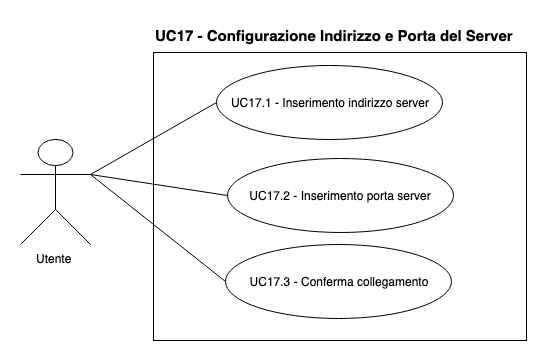
\includegraphics[scale=0.5]{./images/UC17.png}
%	\caption{UC17 - Configurazione Indirizzo e Porta del Server.}
%\end{figure}
\begin{itemize}
	\item \textbf{Attore Primario:} Utente
	\item \textbf{Precondizione:}
	\begin{enumerate}
		\item L'utente ha aggiunto il pannello "G\&B" alla propria dashboard;
		\item L'utente ha avviato il monitoraggio (\hyperref[UC20]{UC20(§\ref*{UC20})}).
	\end{enumerate}
	\item \textbf{Postcondizione:} L'utente ha interrotto il monitoraggio precedentemente attivo.
	\item \textbf{Scenario Principale:}
	\begin{enumerate}
		\item L'utente interrompe il monitoraggio della rete le cui impostazioni sono attualmente visualizzate attraverso il click del bottone con etichetta "Interrompi Monitoraggio".
	\end{enumerate}
\end{itemize}

\pagebreak

\subsection{UC22 - Visualizzazione Errore nel Collegamento al Server}\label{UC22}
%\begin{figure}[H]
%	\centering
%	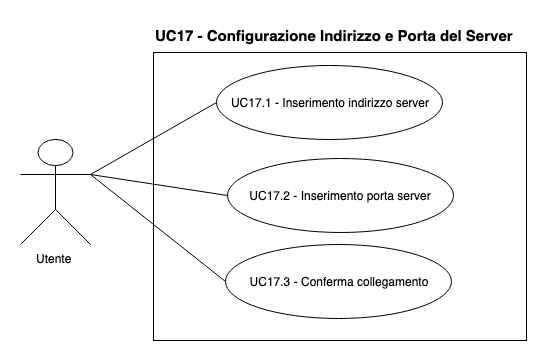
\includegraphics[scale=0.5]{./images/UC17.png}
%	\caption{UC17 - Configurazione Indirizzo e Porta del Server.}
%\end{figure}
\begin{itemize}
	\item \textbf{Attore Primario:}  Utente
	\item \textbf{Precondizione:}
	\begin{enumerate}
		\item L'utente ha cliccato il pulsante con etichetta "Collega" per confermare il collegamento al server con i dati precedentemente impostati (\hyperref[UC17]{UC17 (§\ref*{UC17})}).
	\end{enumerate}
	\item \textbf{Postcondizione:} L'utente ha visualizzato il messaggio di errore;
	\item \textbf{Scenario Principale:}
	\begin{enumerate}
		\item L'utente visualizza l'errore di collegamento;
		\item L'utente clicca "OK".
	\end{enumerate}
\end{itemize}

\pagebreak

\subsection{UC23 - Selezione Rete Bayesiana già caricata}\label{UC23}
%\begin{figure}[H]
%	\centering
%	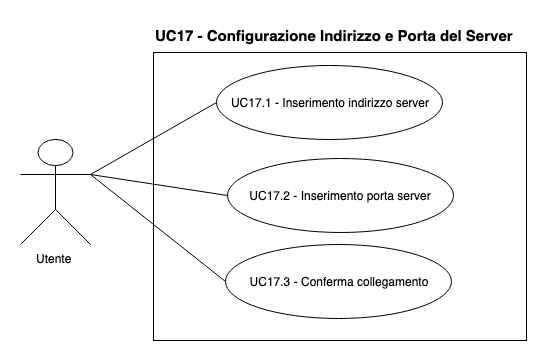
\includegraphics[scale=0.5]{./images/UC17.png}
%	\caption{UC17 - Configurazione Indirizzo e Porta del Server.}
%\end{figure}
\begin{itemize}
	\item \textbf{Attore Primario:}  Utente
	\item \textbf{Precondizione:} L'utente ha correttamente configurato le impostazioni per la connessione al server \hyperref[UC17]{UC17(§\ref*{UC17})};
	\item \textbf{Postcondizione:}
	\begin{enumerate}
		\item L'utente visualizza le impostazioni della rete selezionata;
		\item Se la rete non è in fase di monitoraggio, il cambio della rete porta al salvataggio di questa nel server;
	\end{enumerate}
	\item \textbf{Scenario Principale:}
	\begin{enumerate}
		\item L'utente apre il menù a tendina per la selezione di una rete già precedentemente caricata;
		\item L'utente seleziona la rete.
	\end{enumerate}
\end{itemize}

\subsubsection{UC23.1 - Apertura del Menù a Tendina per la Selezione di una Rete Precedentemente Caricata}\label{UC23.1}
\begin{itemize}
	\item \textbf{Attore Primario:}  Utente
	\item \textbf{Precondizione:}
	\begin{enumerate}
		\item L'utente ha correttamente configurato le impostazioni per la connessione al server \hyperref[UC17]{UC17(§\ref*{UC17})};
		\item L'utente ha correttamente selezionato il database TODO %\hyperref[UC17]{UC17.2 (§\ref*{UC17.2})}.
	\end{enumerate}
	\item \textbf{Postcondizione:} l'utente ha aperto il menù a tendina per la selezione di una rete precedentemente caricata;
	\item \textbf{Scenario Principale:} l'utente clicca sul menù a tendina "Selezione Reti Caricate" per la selezione di una rete  precedentemente caricata.
\end{itemize}

\subsubsection{UC23.2 - Selezione della Rete Precedentemente Caricata}\label{UC23.2}
\begin{itemize}
	\item \textbf{Attore Primario:} Utente
	\item \textbf{Precondizione:}  l'utente ha aperto il menù a tendina "Selezione Reti Caricate" \hyperref[UC23.1]{UC23.1 (§\ref*{UC23.1})}
	\item \textbf{Postcondizione:} l'utente ha selezionato la rete dal menù a tendina "Selezione Reti Caricate";
	\item \textbf{Scenario Principale:} l'utente seleziona, dal menù a tendina, una rete precedentemente caricata per avviarne il monitoraggio.
\end{itemize}

\pagebreak

\subsection{UC26 - Visualizzazione Notifica di Avvenuto Collegamento al Server}\label{UC26}
%\begin{figure}[H]
%	\centering
%	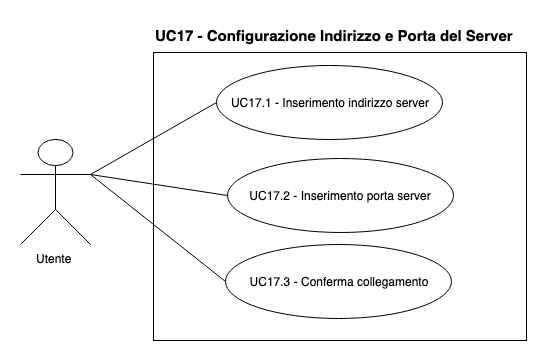
\includegraphics[scale=0.5]{./images/UC17.png}
%	\caption{UC17 - Configurazione Indirizzo e Porta del Server.}
%\end{figure}
\begin{itemize}
	\item \textbf{Attore Primario:}  Utente
	\item \textbf{Precondizione:}
	\begin{enumerate}
		\item L'utente ha cliccato il pulsante con etichetta "Collega" per confermare il collegamento al server con i dati precedentemente impostati (\hyperref[UC17]{UC17 (§\ref*{UC17})}).
	\end{enumerate}
	\item \textbf{Postcondizione:} L'utente visualizza la notifica dell'avvenuto collegamento;
	\item \textbf{Scenario Principale:}
	\begin{enumerate}
		\item L'utente visualizza il messaggio dell'avvenuto collegamento;
		\item L'utente clicca "OK".
	\end{enumerate}
\end{itemize}


\pagebreak
\rhead{\rightmark}

\section{Requisiti}\label{Requisiti}

\subsection{Requisiti Funzionali}\label{RF}
\begin{center}
\begin{longtable}[c]{|m{.11\textwidth}|m{.50\textwidth}|m{.2\textwidth}|m{.08\textwidth}|}
\hline
\rowcolor{bluelogo}\textbf{\textcolor{white}{ID}} & \textbf{\textcolor{white}{Descrizione}} & \textbf{\textcolor{white}{Obbligatorietà}} & \textbf{\textcolor{white}{Fonti}}\\
\hline \hline
\endhead
ROF1 & L'utente deve poter aggiungere una rete bayesiana al sistema & Obbligatorio & UC1\\
\hline
\rowcolor{grigio}ROF1.1 & Il Sistema deve mettere a disposizione un pulsante per avviare l'operazione di selezione del file da caricare & Obbligatorio & UC1\\
\hline
ROF1.2 & Il Sistema deve consentire all'utente di selezionare un file da caricare & Obbligatorio & UC1\\
\hline
\rowcolor{grigio}ROF1.3 & Il Sistema deve mettere a disposizione dell'utente un bottone per avviare l'operazione di caricamento & Obbligatorio & UC1\\
\hline
ROF1.4 & Il Sistema deve visualizzare un messaggio di errore nel caso l'operazione di caricamento del file non sia andata a buon fine & Obbligatorio & UC1 UC8\\
\hline
\rowcolor{grigio}RFF1.4.1 & Il Sistema deve visualizzare un messaggio di errore nel caso in cui l'estensione del file selezionato sia errata & Opzionale & UC1 UC8\\
\hline
RFF1.4.2 & Il Sistema deve visualizzare un messaggio di errore nel caso in cui la struttura interna del file selezionato sia errata & Opzionale & UC1 UC8\\
\hline
\rowcolor{grigio}ROF2 & L'utente deve poter collegare un flusso di dati ad ogni nodo desiderato della rete preesistente & Obbligatorio & UC2\\
\hline
ROF2.1 & Il Sistema deve interpretare la rete bayesiana caricata, al fine di estrapolarne i nodi e fornirli all'utente sotto forma di lista & Obbligatorio & UC2\\
\hline
\rowcolor{grigio}ROF2.1.1 & Il Sistema deve mostrare, per ogni nodo, il nominativo dello stesso & Obbligatorio & UC2\\
\hline
ROF2.1.2 & Il Sistema deve mostrare, per ogni nodo, una corrispondente checkbox che identifichi lo stato dello stesso: Collegato ad un flusso dati oppure no & Obbligatorio & UC2\\
\hline
\rowcolor{grigio}ROF2.2 & Il Sistema deve mettere a disposizione dell'utente una lista di flussi dati a cui collegare i nodi desiderati & Obbligatorio & UC2\\
\hline
ROF2.2.1 & Il Sistema, in seguito al click dell'utente su un nominativo, deve aprire una finestra contente un elenco dei flussi dati disponibili per il collegamento & Obbligatorio & UC2\\
\hline
\rowcolor{grigio}ROF2.2.2 & L'utente deve poter cliccare il flusso dati desiderato per il collegamento & Obbligatorio & UC2\\
\hline
ROF2.3 & L'utente deve poter definire, per ogni nodo che ha deciso di collegare ad un flusso dati, un livello di soglia, al di sotto, o al di sopra del quale si verifichi l'evidenza dell'evento all'interno della rete bayesiana & Obbligatorio & UC2\\
\hline
\rowcolor{grigio}ROF2.4 & Il Sistema deve mettere a disposizione dell'utente un bottone per confermare il collegamento dei nodi & Obbligatorio & UC2\\
\hline
ROF2.5 & Il Sistema deve visualizzare un messaggio di errore nel caso in cui l'utente abbia confermato il collegamento dei nodi senza averne effettivamente collegato alcuno & Obbligatorio & UC2 UC9\\
\hline
\rowcolor{grigio}ROF2.6 & Il Sistema deve aggiornare la lista di checkbox, registrando il nuovo stato di ogni nodo (collegato o meno ad un flusso dati) & Obbligatorio & UC2\\
\hline
ROF3 & L'utente deve poter impostare una policy per il ricalcolo delle probabilità nella rete & Obbligatorio & UC3\\
\hline
\rowcolor{grigio}ROF3.1 & L'utente deve avere la possibilità di impostare una policy esistente ad una rete bayesiana  & Obbligatorio & UC3\\ 
\hline
ROF3.2 & L'utente deve avere la possibilità di creare una nuova policy da aggiungere ad una rete bayesiana & Obbligatorio & UC3\\
\hline
\rowcolor{grigio}ROF4 & Il Sistema deve fornire i dati relativi ai nodi della rete bayesiana non collegati al flusso & Obbligatorio & UC4\\
\hline
ROF4.1 & Il Sistema deve fornire all'utente una lista di probabilità dinamiche associate ai nodi della rete & Obbligatorio & UC4\\
\hline
\rowcolor{grigio}ROF4.2 & Il Sistema deve aggiornare periodicamente le probabilità in base a quanto definito come policy per il ricalcolo delle probabilità & Obbligatorio & UC4\\
\hline
ROF4.3 & Il Sistema deve mettere a disposizione di \textit{Grafana} i dati per l'operazione di creazione di alert ad essi associati da parte dell'utente & Obbligatorio & UC5\\
\hline
\rowcolor{grigio}ROF5 & Il Sistema deve mostrare all'utente gli alert associati al flusso di dati collegato alla rete bayesiana & Obbligatorio & UC7\\ 
\hline
ROF5.1 & L'utente deve poter rimuovere gli alert associati ai nodi della rete bayesiana & Obbligatorio & UC6\\ 
\hline
\caption{Requisiti Funzionali}
\end{longtable}
\end{center}


%\subsection{Requisiti Prestazionali}\label{RP}

\subsection{Requisiti di Qualità}\label{RQ}
\begin{center}
\begin{longtable}[c]{|m{.09\textwidth}|m{.48\textwidth}|m{.2\textwidth}|m{.12\textwidth}|}
\hline
\rowcolor{bluelogo}\textbf{\textcolor{white}{ID}} & \textbf{\textcolor{white}{Descrizione}} & \textbf{\textcolor{white}{Obbligatorietà}} & \textbf{\textcolor{white}{Fonti}}\\
\hline \hline
\endhead
ROQ1 & E' necessario fornire un manuale utente, per l'utilizzo del prodotto, in formato \textit{pdf} & Obbligatorio & Capitolato\\
\hline
\rowcolor{grigio}ROQ1.1 & Il manuale utente deve essere disponibile in lingua italiana & Obbligatorio & Decisione Interna\\
\hline
RDQ1.2 & Il manuale utente deve essere disponibile in lingua inglese & Desiderabile & Decisione Interna\\
\hline
\rowcolor{grigio}ROQ2 & E' necessario fornire un manuale per la manutenzione ed estensione del prodotto & Obbligatorio & Capitolato\\
\hline
ROQ2.1 & Il manuale di manutenzione/estensione deve essere disponibile in lingua italiana & Obbligatorio & Decisione Interna\\
\hline
\rowcolor{grigio}RDQ2.2 & Il manuale di manutenzione/estensione deve essere disponibile in lingua inglese & Desiderabile & Decisione Interna\\
\hline
ROQ3 & Il prodotto deve essere sviluppato in modo concorde a quanto stabilito nelle \textit{Norme di Progetto v1.0.0} & Obbligatorio & Decisione Interna\\
\hline
\caption{Requisiti di Qualità}
\end{longtable}
\end{center}



\subsection{Requisiti di Vincolo}\label{RV}
\begin{center}
\begin{longtable}[c]{|m{.1\textwidth}|m{.53\textwidth}|m{.25\textwidth}|}
\hline
\rowcolor{bluelogo}\textbf{\textcolor{white}{ID}} & \textbf{\textcolor{white}{Descrizione}} & \textbf{\textcolor{white}{Fonti}}\\
\hline \hline
\endfirsthead
ROV1 & Il plug-in deve essere sviluppato in linguaggio \textit{ECMAScript6} & \textit{Grafana}: guida per gli sviluppatori\\
\hline
\rowcolor{grigio}ROV2 & Il punto di ingresso per il plug-in deve essere sviluppato nel file "module.js" & \textit{Grafana}: guida per gli sviluppatori\\
\hline
ROV3 & Va utilizzato un qualsiasi build system\glossario che supporti \textit{systemjs}\glossario & \textit{Grafana}: guida per gli sviluppatori\\
\hline
\caption{Requisiti di Vincolo}
\end{longtable}
\end{center}
\pagebreak

\subsection{Tacciamento Fonti-Requisiti}\label{Tracciamento}
\begin{center}
\begin{longtable}[c]{|c|m{.15\textwidth}|}
\hline
\rowcolor{bluelogo}\textbf{\textcolor{white}{Fonte}} & \textbf{\textcolor{white}{Requisiti}}\\
\hline \hline
\endhead
Capitolato & \makecell{ROQ1\\ROQ2}\\
\hline
\rowcolor{grigio}Decisione Interna & \makecell{ROQ1.1\\RDQ1.2\\ROQ2.1\\RDQ2.2\\ROQ3}\\
\hline
Piattaforma \textit{Grafana} & \makecell{ROV1\\ROV2\\ROV3}\\
\hline
\rowcolor{grigio}UC1 & \makecell{ROF1\\ROF1.1\\ROF1.2\\ROF1.3\\ROF1.4\\RFF1.4.1\\RFF1.4.2}\\
\hline
UC2 & \makecell{ROF2\\ROF2.1\\ROF2.1.1\\ROF2.1.2\\ROF2.2\\ROF2.2.1\\ROF2.2.2\\ROF2.3\\ROF2.4\\ROF2.5\\ROF2.6}\\
\hline
\rowcolor{grigio}UC3 & \makecell{ROF3\\ROF3.1\\ROF3.2}\\
\hline
UC4 & \makecell{ROF4\\ROF4.1\\ROF4.2}\\
\hline
\rowcolor{grigio}UC5 & \makecell{ROF4.3}\\
\hline
UC6 & \makecell{ROF5.1}\\
\hline
\rowcolor{grigio}UC7 & \makecell{ROF5}\\
\hline
UC8 & \makecell{ROF1.4\\RFF1.4.1\\RFF1.4.2}\\
\hline
\rowcolor{grigio}UC9 & \makecell{ROF2.5}\\
\hline
\caption{Tracciamento Fonti-Requisiti}
\end{longtable}
\end{center}


\subsection{Riepilogo Requisiti}\label{Riepilogo}
\begin{center}
\begin{longtable}[c]{|c|c|c|c|c|}
\hline
\rowcolor{bluelogo}\textbf{\textcolor{white}{Tipologia}} & \textbf{\textcolor{white}{Obbligatorio}} & \textbf{\textcolor{white}{Opzionale}} & \textbf{\textcolor{white}{Desiderabile}} & \textbf{\textcolor{white}{Totale}}\\
\hline \hline
\endhead
Funzionale & 25 & 2 & 0 & 27\\
\hline
\rowcolor{grigio}Di Qualità & 5 & 0 & 2 & 7\\
\hline
Di Vincolo & 3 & 0 & 0 & 3\\
\hline
\caption{Riepilogo dei Requisiti}
\end{longtable}
\end{center}

\end{document}